\documentclass[11pt]{article}

\usepackage[T1]{fontenc}
\usepackage{mathptmx}
\usepackage{graphicx}

\topmargin 0.0in
\setlength{\textwidth} {420pt}
\setlength{\textheight} {620pt} 
\setlength{\oddsidemargin} {20pt}
\setlength{\marginparwidth} {72in}

\usepackage{fancyhdr} 
\usepackage{url}

% set it so that subsubsections have numbers and they
% are displayed in the TOC (maybe hard to read, might want to disable)

\setcounter{secnumdepth}{3}
\setcounter{tocdepth}{3}

% define widow protection

\def\widow#1{\vskip #1\vbadness10000\penalty-200\vskip-#1}

\clubpenalty=10000  % Don't allow orphans
\widowpenalty=10000 % Don't allow widows

% this should give me the ability to use some math symbols that 
% were available by default in standard latex (i.e. \Box)

\usepackage{latexsym}

% define a little section heading that doesn't go with any number

\def\littlesection#1{
\widow{2cm}
\vskip 0.5cm
\noindent{\bf #1}
\vskip 0.0001cm 
}

\pagestyle{fancyplain}

\newcommand{\tstamp}{\today}   
\renewcommand{\sectionmark}[1]{\markright{#1}}
\lhead[\Section \thesection]            {\fancyplain{}{\rightmark}}
\chead[\fancyplain{}{}]                 {\fancyplain{}{}}
\rhead[\fancyplain{}{\rightmark}]       {\fancyplain{}{\thepage}}
\cfoot[\fancyplain{\thepage}{}]         {\fancyplain{\thepage}{}}

\newlength{\myVSpace}% the height of the box
\setlength{\myVSpace}{1ex}% the default, 
\newcommand\xstrut{\raisebox{-.5\myVSpace}% symmetric behaviour, 
  {\rule{0pt}{\myVSpace}}%
}

% leave things with no spacing extra spacing in the final version of the paper
\renewcommand{\baselinestretch}{1.0}    % must go before the begin of doc

% suppress the use of indentation for a paragraph

\setlength{\parindent}{0.0in}
\setlength{\parskip}{0.1in}
\setlength{\headheight}{15pt}

\begin{document}

%% \begin{abstract}

%%   Try

%% \end{abstract}

% handle widows appropriately
\def\widow#1{\vskip #1\vbadness10000\penalty-200\vskip-#1}

% build the title section

\makeatletter

\def\maketitle{%
  %\null
  \thispagestyle{empty}%
  %\vfill
  \begin{center}%\leavevmode
    %\normalfont
    {\Huge \@title\par}%
    %\hrulefill\par
    {\normalsize \@author\par}%
    \vskip .4in
%    {\Large \@date\par}%
  \end{center}%
  %\vfill
  %\null
  %\cleardoublepage

  }

\makeatother

\vspace*{-1.1in}
\title{Contextual Gesture Correction and Recognition}

% build the author section
\author{Braden D. Licastro\\
Department of Computer Science\\
Allegheny College \\
{\tt licastb@allegheny.edu}  \\
\url{http://www.fullforceapps.com/} \\ 
\vspace*{.1in} \today \\ \vspace*{.1in}
{\bf Abstract} \\ This paper describes a method of generating a correct response to a touch screen gesture that would normally produce incorrect results. Currently touch screen devices use techniques such as voice pattern matching and predictive text to improve user experience, but this leaves other areas for improvement. This research would develop a system that can look at a provided gesture and choose a best-guess action based on similar pre-programmed gestures, or make a prediction based on either previous choices by the user.}

% use the default title stuff
\maketitle

\vspace*{-.4in}
\section{Introduction}
\label{sec:introduction}
\vspace*{-.1in}

As touch devices become more widely used the technology must advance to keep up with the needs of the users. The two main types of commonly used touch devices both allow a user to use either a stylus or their finger. This can mean vastly different code depending what is being used which adds complexity to an already difficult situation. Along with different technologies being available for the hardware itself, user input can greatly vary. Many devices utilize gyroscopes, magnetic sensors, GPS units, proximity sensors, light sensors, and much more to allow the user to seamlessly interact with the device. Although these can be used to broaden the spectrum of possible interactions, the use is varied at best, and often overlooked. 

The most versatile method of input acceptance is a users hand. With five fingers and a virtually unlimited number of possible motions, finger input is the most commonly used. Due to the variations on shape, size, and accuracy of people's hands and motions this makes programming gestures difficult. Currently devices are very forgiving of error, some to the point where any gesture at all will be matched with an action, whether correct or not. This can lead to use frustration, which can cause additional trouble with input when flustered. Keyboards are beginning to be coded to allow for adaptability. They are coded to adjust the active area over the buttons to correspond with common placement of a users fingers on the screen. This is correcting for per user error. This can also be seen in other implementations as described in the Related Work section. If it is being done in other ways, why not implement a similar function with movement gestures instead?

\vspace*{-.1in}
\section{Related Work}
\label{sec:relatedwork}
\vspace*{-.1in}

The topic of gesture correction and recognition is a very new research topic. There is currently no research that directly correlates to the topic, but there is a small amount that can be used to build a working program. To begin, fuzzy logic algorithm research has been performed and yielded very reliable results with gesture recognition\cite{Anderson:2004:VFL:1067343.1067382}. The paper discusses a system where a video camera is used in conjunction with a low cost, electronics free wand\cite{Anderson:2004:VFL:1067343.1067382}. Because a non-electronic wand is being used to create the users gestures, this will relate directly to a touch screen. The tip of the wand is tracked in a manner very similar to how a finger is tracked on a screen.

To prove their findings, the authors used two different sets of hardware that were user trained by recording gestures, and on the commercially available hardware they used a reference set of gestures that were hard coded into the software. This returned interesting results, but proved that the gestures can be used cross platform, but with an increase in recognition failure as seen in the figure they provided.

\begin{center}
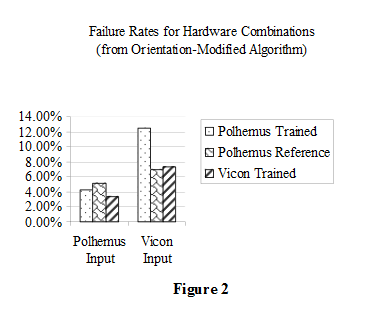
\includegraphics[scale=.8]{hardwarerelation}
\end{center}

In addition, the authors provided an overall failure rate of the systems and various implementations of their algorithms. They concluded that the fuzzy logic algorithm with weight and orientation both modified performed significantly than the original, or even just having one variable modified. This is important as the average failure rate is in the single digits as seen in the graph.

\begin{center}
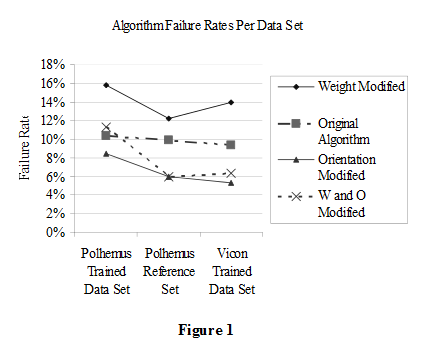
\includegraphics[scale=.8]{failurerate}
\end{center}

In addition to to the research paper previously mentioned, the last that could benefit this research is only loosely related. The authors proposed an approach to identifying gesture patterns before they are complete by analyzing previously recorded gestures and finding related actions that immediately follow. \cite{Shimada:2010:ERB:1939751.1939810} The paper doesn't provide any concrete evidence or numbers to verify their hypothesis, but instead discusses the probability that such a system is feasible. In addition to matching gesture patterns and repeated occurrence of other actions immediately following said gesture, the authors also discuss relationships between multiple users on the same device. This is where the topic no longer follows the research I propose. The writer assumes that both users are interacting with the device having the same goal in mind, which would allow the same gesture pattern to be used. In the case of the proposed research, either one user would be linked to a gesture profile, or they would have to be generic enough to work across a vast number of users.

\vspace*{-.2in}
\section{Method of Approach}
\label{sec:method}
\vspace*{-.1in}

The proposed research will entail creating a program that is capable of recognizing gestures as outlined. In addition, some way of determining correct and incorrect gestures must be implemented. To evaluate the algorithms and user history tracking, an android touch enabled device will need to be acquired that is compatible with the proposed program.

The software itself will be created using the Java language, and the Gesture Coder module for the Eclipse programming environment. Gesture Coder will be used to create the base cases for the gestures in order to decrease development time.

\begin{center}
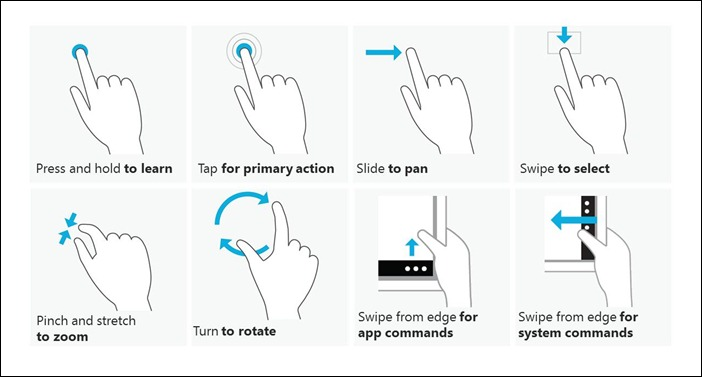
\includegraphics[scale=.5]{gestures}
\end{center}

From these base gestures, as pictured in the provided figure, the software will begin to adapt the code to accept either a broader spectrum of variances of the gesture, or it will learn a specific motion that a user inputs when trying to instruct the device to perform a specific function.

To determine whether a gesture is incorrectly identified by the software, several approaches will be used. The most straightforward would be a camera recording their facial expressions. As a user is testing the device a confused or frustrated expression would be a key indicator that a gesture was incorrectly chosen by the software. This would be considered a failure. In addition, as a user interacts with the device, many consecutive movements that are very similar can be used as an indicator that the program incorrectly identified the motion. In this case the user may either repeat the exact same motion, or vary it slightly. Lastly, there will be a option in the testbed that would allow the user to give up on a command and choose an option saying that the software could not respond in a manner similar to what they needed.


\vspace*{-.2in}
\section{Evaluation Strategy}
\label{sec:evaluate}
\vspace*{-.1in}

In order to gather accurate data, the software will include several features. Most important, the program will be able to calculate a fitness for each input gesture. The closer to '1' that it gets, the more similar to a predefined gesture it is. If the user inputs many gestures that are similar, and have nearly identical fitness values the program will prompt the user asking whether it has failed to accurately choose an action from their gesture and the response will be recorded.

Before the test begins, the test subjects will have exactly 5 minutes to look over a set of multi part commands and remember them as well as possible. During the test a user will have an option to glance for several seconds if they cannot recall the gesture, but they must not be given an opportunity to memorize the exact movement. When the device asks them to perform a specific action, they may or may not recall the exact gesture, and the error introduced will allow the software to use its logic to correct for this and choose the correct action. The program will not know what will be asked of the user as the questions will be separate from the algorithms, and the results will be collected by the questionnaire.

Lastly, in order to give the user some way of bypassing a question that the software cannot complete successfully, the user will get 10 separate opportunities to retry the gesture, or the option to fail the question after five attempts.

\vspace*{-.1in}
\section{Research Schedule}
\label{sec:schedule}
\vspace*{-.1in}

To begin the project several topics must be addressed, namely development process, method of installation, data collection, and the data evaluation itself. Within the first two to four weeks of beginning the project I will research the availability and features of various touch enabled devices and find one which is best suited for this research. In addition, accompanying programs will be coded that record various metrics relating to the test subjects experience. 

Phase 1 - 1 week: To begin the research process I will choose a device in which I will be running the test program on and choose the subjects whom I feel will be best suited for this research. People with minimal experience using this type of computing device will be used as predefined gestures on other devices will not be able to interfere with results.

Phase 2 - 2-3 months: Develop a working program which is able to successfully read input gestures and perform a function dependent on what the gesture is. It should be able to determine a best fit action based on the users past interactions in a similar environment and the programs ability to match vague or partially incorrect gestures.

Phase 3 - 2 weeks: During this time I will run various tests on the software using correct, incorrect, and similar gestures to what are hard coded into the software. This time period will allow for minor code adjustments and initial benchmarks before the software begins to learn gesture variations.

Phase 4 - 1 week: This is the official testing phase. During this week I will bring in test subjects for 1 hour each and allow them to use the tablet by matching gestures that the software flashes at them for three seconds. This will allow the user to get used to the feel of the device, and will allow the software to build a database of minor variances that the users commonly make when using these gestures, such as an orientation change or wavy lines when attempting to draw a straight line.

The subjects will be brought back a second time to test the device using the gesture sets they are unfamiliar with and test data will be evaluated from these.

Phase 5 - remaining time: The remaining time will be used to evaluate facial expression recordings and the data returned per user by the software. From this it can be determined whether the software successfully completed its task and details such as failure rates, repeated attempts to input gestures and so on.

\vspace*{-.1in}
\section{Conclusion}
\label{sec:conclusion}
\vspace*{-.1in}

As the use of touch enabled devices becomes more commonplace the technology is going to evolve and become more complex. The number of gestures will increase as more complex software is introduced which will lead to user frustration and confusion. By developing a system capable of evaluating a best fit action for a specific gesture and software environment, the time and energy spent trying to make a device cooperate can be greatly reduced. It may be possible to further extend the research proposed and include the ability to custom record gestures for specific functions, or even re-purpose existing gestures to something the user finds more intuitive. In addition, due to the use of context based gesture evaluation it is possible that one gesture can perform multiple tasks if a user frequently performs the same task repeatedly. 

\bibliographystyle{plain}
\bibliography{senior_thesis_proposal}

\end{document}

